\documentclass[a4paper,12pt]{article}

\usepackage{cmap}					
\usepackage[T2A]{fontenc}			
\usepackage[utf8]{inputenc}			
\usepackage[english,russian]{babel}	

\usepackage{amsmath,amsfonts,amssymb,amsthm,mathtools} 
\usepackage{wasysym}


\usepackage{graphicx}
\usepackage[cache=false]{minted}

\usepackage{indentfirst}
\usepackage{amssymb}


\usepackage{listings} 
\usepackage{fancyvrb}
%\DefineShortVerb{\|}

\usepackage{color}
\usepackage{caption}
\DeclareCaptionFont{white}{\color{black}}
\DeclareCaptionFormat{listing}{\colorbox{white}{\parbox{\textwidth}{#1#2#3}}}
\captionsetup[lstlisting]{format=listing,labelfont=white,textfont=white}


\usepackage{listings}

\usepackage{geometry}
\geometry{left=2cm}
\geometry{right=1.5cm}
\geometry{top=1cm}
\geometry{bottom=2cm}
\setlength{\parindent}{5ex}
\setlength{\parskip}{0.5em}

\begin{document} % Конец преамбулы, начало текста.

\lstset{ %
language=C++,                 % выбор языка для подсветки (здесь это С)
basicstyle=\small\sffamily, % размер и начертание шрифта для подсветки кода
numbers=left,               % где поставить нумерацию строк (слева\справа)
numberstyle=\tiny,           % размер шрифта для номеров строк
stepnumber=1,                   % размер шага между двумя номерами строк
numbersep=5pt,                % как далеко отстоят номера строк от подсвечиваемого кода
backgroundcolor=\color{white}, % цвет фона подсветки - используем \usepackage{color}
showspaces=false,            % показывать или нет пробелы специальными отступами
showstringspaces=false,      % показывать или нет пробелы в строках
showtabs=false,             % показывать или нет табуляцию в строках
frame=single,              % рисовать рамку вокруг кода
tabsize=2,                 % размер табуляции по умолчанию равен 2 пробелам
captionpos=t,              % позиция заголовка вверху [t] или внизу [b] 
breaklines=true,           % автоматически переносить строки (да\нет)
breakatwhitespace=false, % переносить строки только если есть пробел
escapeinside={\%*}{*)}   % если нужно добавить комментарии в коде
}


\large
\begin{center}
Федеральное государственное бюджетное образовательное учреждение высшего образования «Московский государственный технический университет имени Н. Э. Баумана (национальный исследовательский университет»)
\end{center}

\vspace*{30mm} 

\LARGE
\begin{center}
Курс: <<Анализ алгоритмов>>

Лабораторная работа №2
\end{center}

\vspace*{30mm} 

\huge
\begin{center}
Тема работы:\\
<<Умножение матриц>>
\end{center}
\vspace*{30mm} 

\large
\begin{flushright}
Студент: Волков Е. А. \\
Преподаватели: Волкова Л. Л. \\
				Строганов Ю. В. \\
Группа: ИУ7-55Б
\end{flushright}

\vspace*{40mm}
\begin{center}
2019    
\end{center}
\thispagestyle{empty}
\pagebreak


\tableofcontents
\pagebreak


\section*{Введение}
\addcontentsline{toc}{section}{Введение}

Цель лабораторной работы: изучение метода динамического программирования на материале алгоритмов стандартного умножения матриц и умножения матриц по Винограду.

Задачи работы:

	
\begin{enumerate} 
	
	\item[1)] изучение стандартного алгоритма умножения матриц и алгоритма умножения матриц по Винограду;
	\item[2)] оптимизация алгоритма Винограда;
	\item[3)] применение метода динамического программирования для  
	реализации указанных
	алгоритмов;
	\item[4)] практические навыки реализации указанных алгоритмов: стандартного алгоритма умножения и умножения по Винограду в двух реализациях: оптимизированной и неоптимизированной;
	\item[5)] сравнительный анализ алгоритмов по затрачиваемым ресурсам (времени);
	\item[6)] экспериментальное подтверждение различий во временнóй эффективности
	алгоритмов при помощи разработанного программного обеспечения на материале замеров
	процессорного времени на варьирующихся размерностях матриц;
	\item[7)] описание и обоснование полученных результатов в отчете о выполненной
	лабораторной
	работе, выполненного как расчётно-пояснительная записка к работе. 
\end{enumerate} 
\pagebreak



\section{Аналитический раздел}
	
	В данном разделе анализируются алгоритмы вычисления произведения матриц по стандартному алгоритму и алгоритму Винограда. 
	
 
	
	\subsection{Описание алгоритмов}
	Матрица A размера $m \times n$ — это прямоугольная таблица чисел, расположенных в m строках и n столбцах:
	\[A = \begin{pmatrix}
a_{11} & a_{12} & ... & a_{1n}\\
a_{21} & a_{22} & ... & a_{2n}\\
... & ... & ... & ...\\
a_{mn} & a_{m2} & ... & a_{mn}\\
\end{pmatrix} \]
 где $a_{ij} (i = 1, …, m; j =1, …, n)$ — это элементы матрицы A. Первый индекс i — это номер строки, второй индекс j — это номер столбца, на пересечении которых расположен элемент $a_{ij}$~\cite{matr}.
		    
		
	Матрицы широко применяются в математике для компактной записи систем линейных алгебраических или дифференциальных уравнений.
	
	    \subsubsection{Стандартный алгоритм}
	Для вычисления произведения двух матриц каждая строка первой
почленно умножается на каждый столбец второй. Затем подсчитывается сумма таких произведений и записывается в соответствующую клетку результата~\cite{makkonell}:

\[ \begin{bmatrix}
a_{11} & a_{12} & ... & a_{1q}\\
a_{21} & a_{22} & ... & a_{2q}\\
... & ... & ... & ...\\
a_{m1} & a_{m2} & ... & a_{mq}\\
\end{bmatrix} \times 
\begin{bmatrix}
b_{11} & b_{12} & ... & b_{1n}\\
b_{21} & b_{22} & ... & b_{2n}\\
... & ... & ... & ...\\
b_{q1} & b_{q2} & ... & b_{qn}\\
\end{bmatrix} = \]
\[=\begin{bmatrix}
a_{11}*b_{11} + ... + a_{1q}*b_{q1} & ... & ... & a_{11}*b_{1n} + ... + a_{1q}*b_{qn}\\
a_{21}*b_{11} + ... + a_{2q}*b_{q1} & ... & ... & a_{21}*b_{1n} + ... + a_{2q}*b_{qn}\\
... & ... & ... & ...\\
a_{m1}*b_{11} + ... + a_{mq}*b_{q1} & ... & ... & a_{m1}*b_{1n} + ... + a_{mq}*b_{qn}\\
\end{bmatrix}. \]
		     		
		    
	  	\subsubsection{Алгоритм Винограда}
		Если посмотреть на результат умножения двух матриц, то видно,
что каждый элемент в нем представляет собой скалярное произведение
соответствующих строки и столбца исходных матриц. Можно заметить
также, что такое умножение допускает предварительную обработку,
позволяющую часть работы выполнить заранее.
	
	Рассмотрим два вектора $V = (v_1, v_2, v_3, v_4)$ и $W = (w_1, w_2, w_3, w_4)$. Их скалярное произведение равно:
	\[
	 V \cdot W = v_1w_1 + v_2w_2 + v_3w_3 + v_4w_4.
	\]
	
	Это равенство можно представить так:
	\[
	 V \cdot W = (v_1 + w_2) * (w_1 + v_2) + (v_3 + w_4)*(w_3 + v_4) - v_1v_2 - v_3v_4 - w_1w_2 - w_3w_4.
	 \]	 
	 
	Такой подход позволяет вычислять $ - v_1v_2 - v_3v_4$ и $ - w_1w_2 - w_3w_4$ заранее и запомнить для каждой строки первой матрицы и для каждого столбца второй. Также в алгоритме Винограда содержится меньше затратных по времени операций умножения, по сравнению со стандартным\cite{makkonell}.
	

	    
		\subsection*{Вывод}
		\addcontentsline{toc}{subsection}{Вывод}
		В данном разделе были рассмотрены алгоритмы стандартного умножения матриц и алгоритм Винограда, которые решает ту же задачу за меньшее количество операций, путем предварительных вычислений частей произведения и путем использования меньшего количества операции умножения. 


\pagebreak


\section{Конструкторский раздел}
	В данном разделе описываются шаги по оптимизации алгоритма Винограда, содержатся схемы алгоритмов и сравнительный анализ алгоритмов (рассматриваются стандартный алгоритм умножения матриц, неоптимизированный алгоритм Винограда и оптимизированный алгоритм Винограда).
	
    \subsection{Оптимизация алгоритма Винограда}
		Заполнение массива под горизонтальные (вертикальные) произведения:
	\begin{enumerate} 
	\item[1)] замена = на +=;
	\item[2)] замена во внутреннем цикле шага цикла с 1 на 2 $\Rightarrow$ происходит замена j*2 на j.
	\end{enumerate}
	
	Тройной цикл:
	\begin{enumerate} 
	\item[1)] замена = на +=;
	\item[2)] замена в цикле по q шага цикла с 1 на 2 $\Rightarrow$ происходит замена k*2 на k;
	\item[3)] вычисление $q2 = q - 1$ заранее;
	\item[4)] использование буфера для накопления результата по циклу q и занесение результата в $res\_matr[i][j]$ после цикла;
	\item[5)] вычисление горизонтального и вертикального произведения заранее отрицательным.

	\end{enumerate}
	
	Условный переход:
	\begin{enumerate} 
	\item[1)] замена = на +=;
	\item[2)] замена во внутреннем цикле шага цикла с 1 на 2 $\Rightarrow$ происходит замена j*2 на j;
	\item[3)] вычисление q2 = q - 1 заранее.
	\end{enumerate}
        
    \subsection{Разработка алгоритмов}
    
        На рис. \ref{fig:schema_mult_st}, \ref{fig:schema_mult_vin} и \ref{fig:schema_mult_vin_opt} приведены схемы стандартного алгоритма умножения матриц и алгоритма Винограда в оптимизированной и неоптимизированной реализациях.
        
        \begin{figure}[h!]
        	\begin{center}
        		{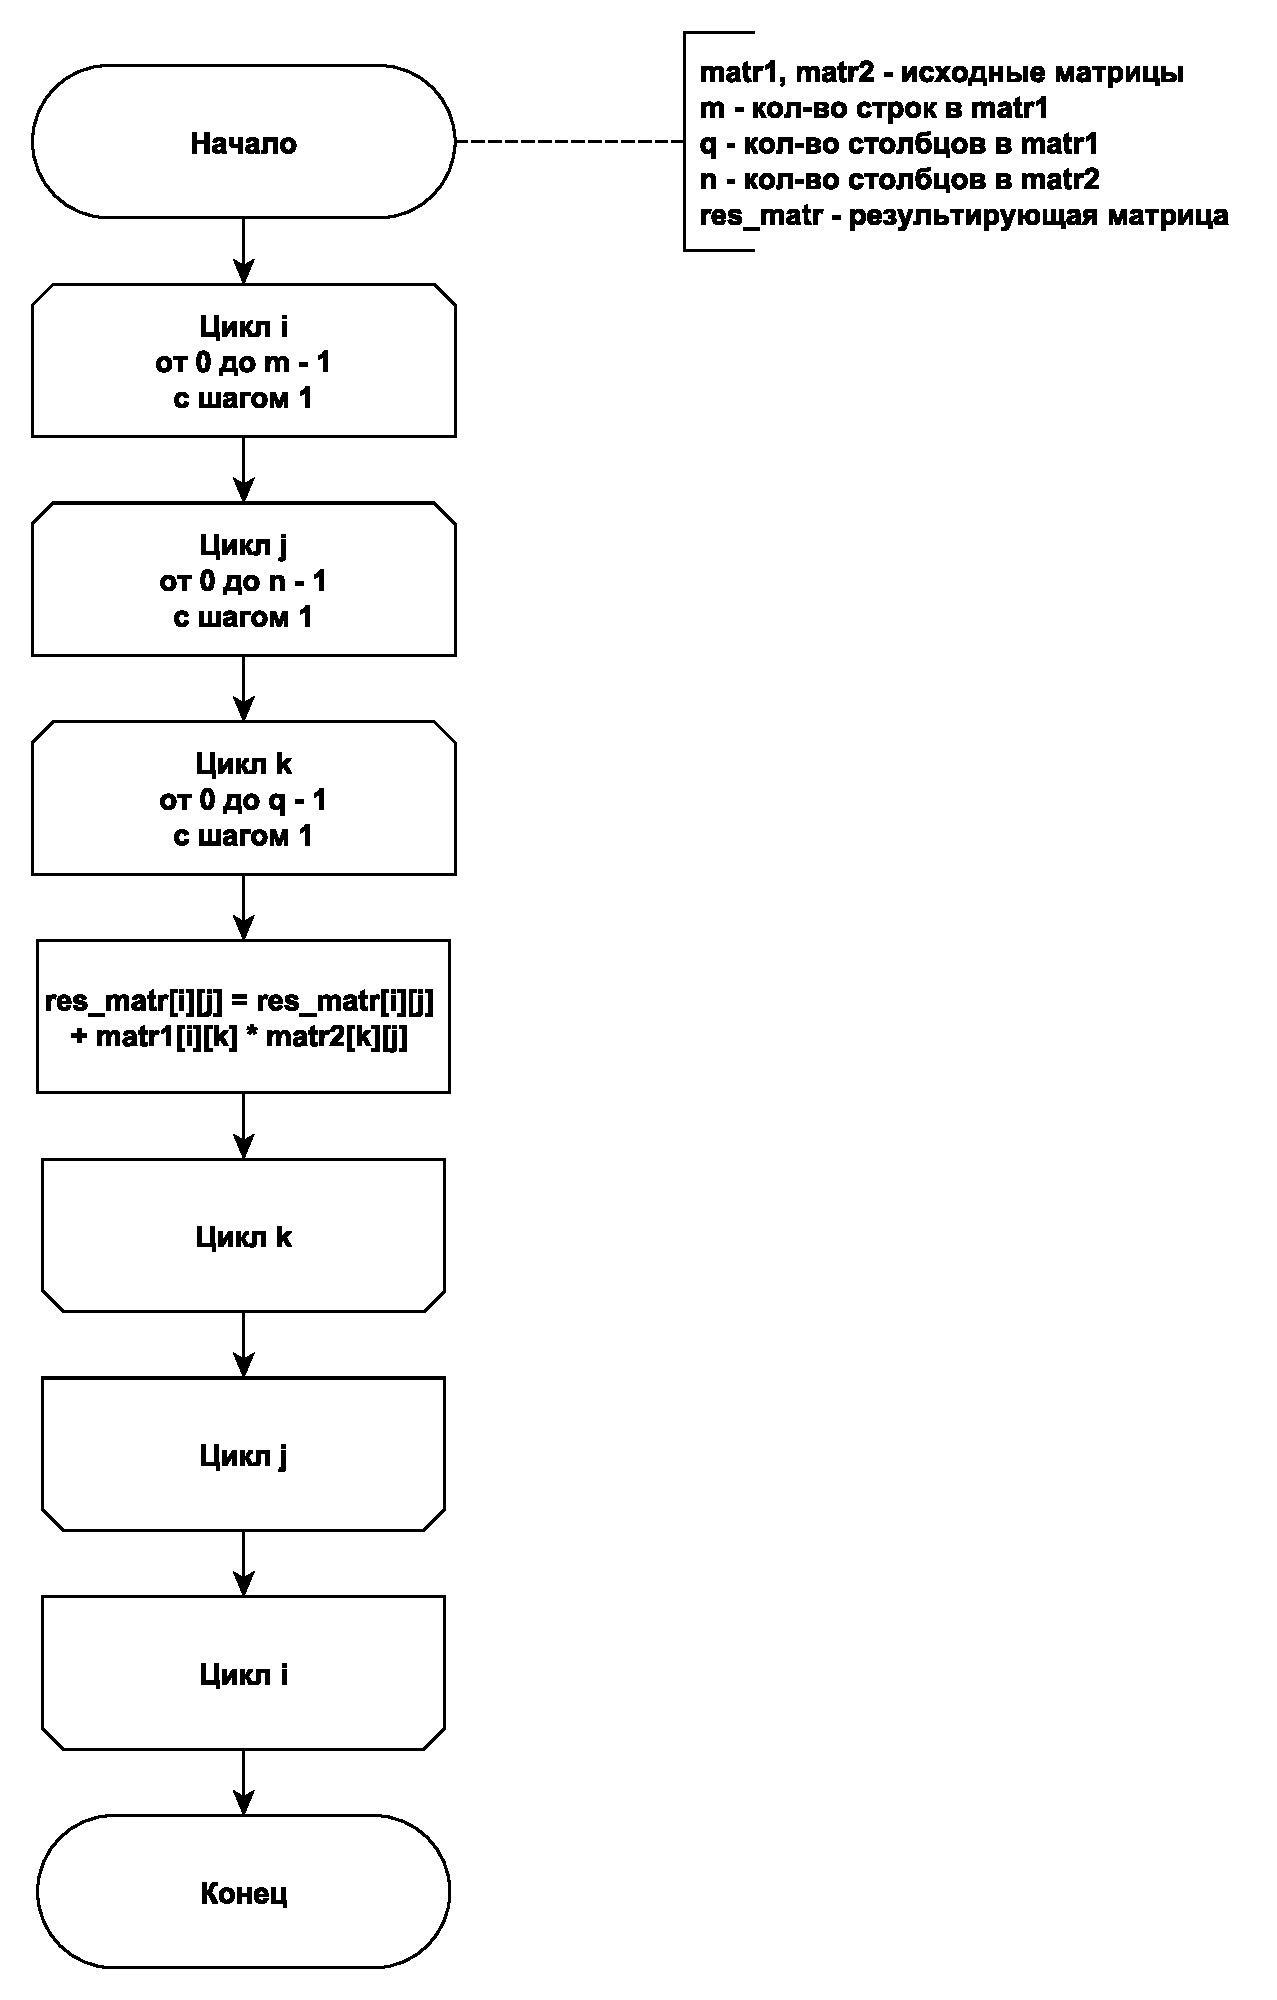
\includegraphics[scale = 0.5]{schema01.pdf}}
        		\caption{Схема стандартного алгоритма умножения матриц}
        		\label{fig:schema_mult_st}
        	\end{center}
        \end{figure}
        
        
        \begin{figure}[h!]
        	\begin{center}
        		{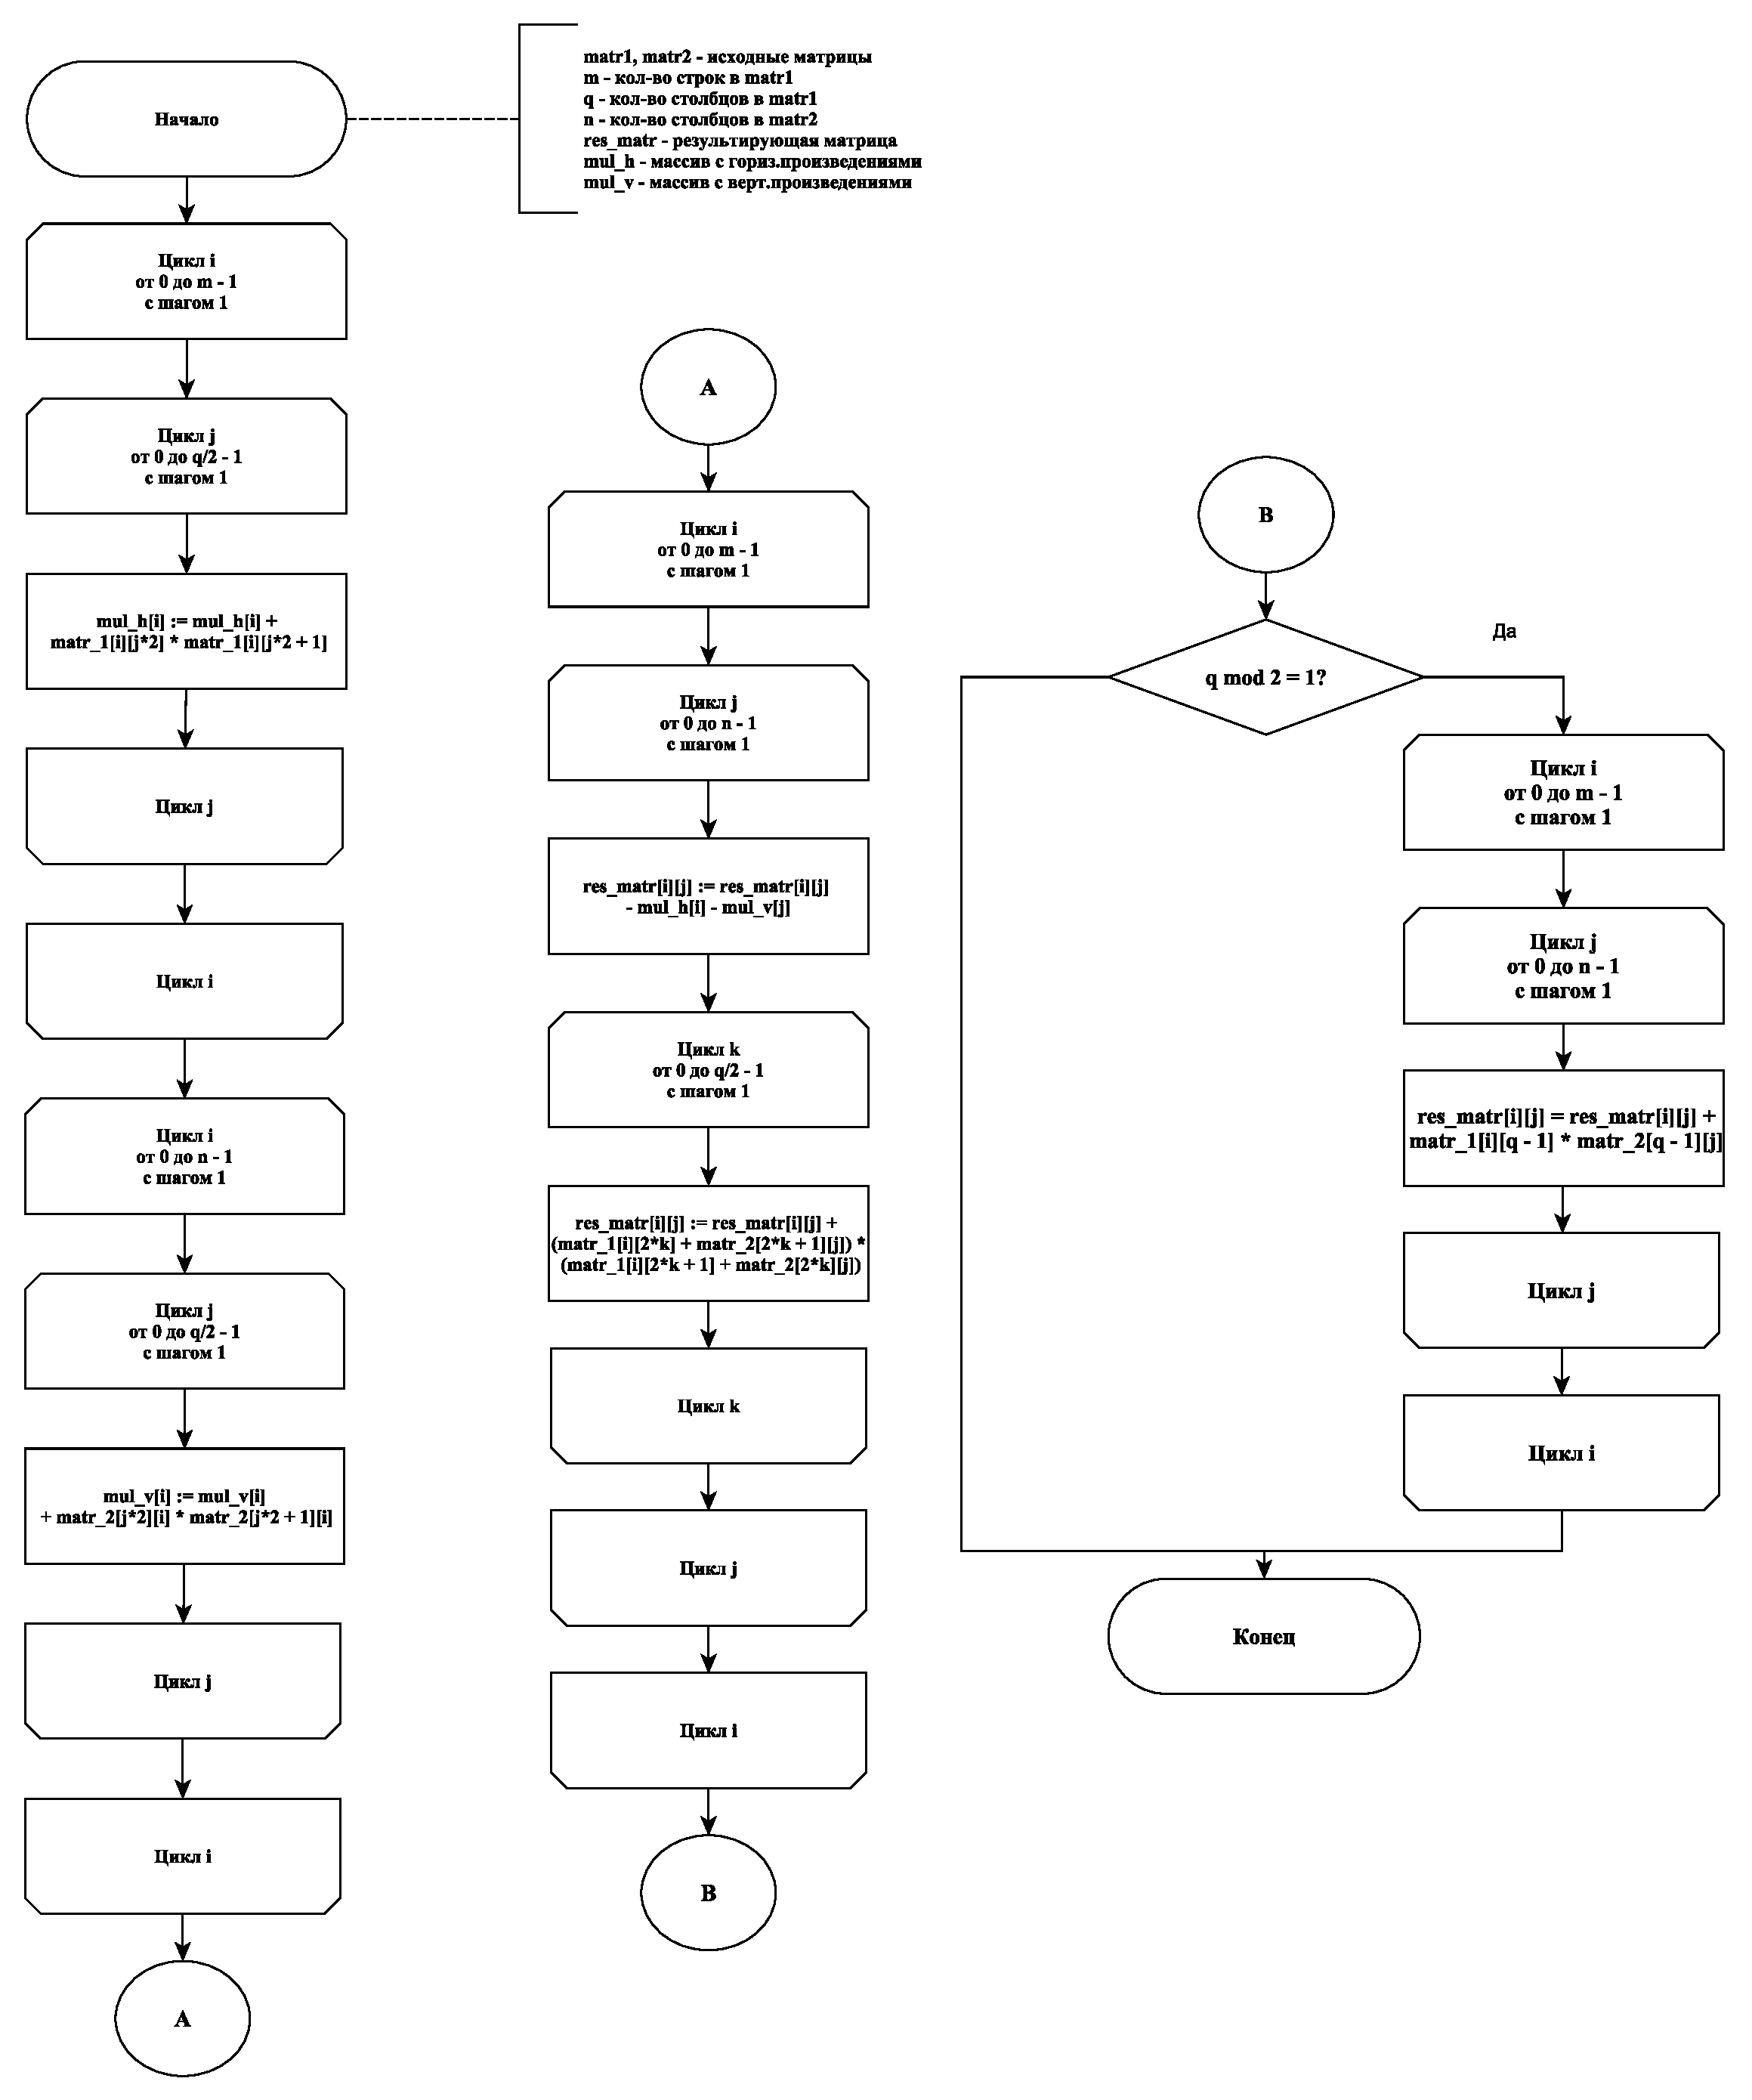
\includegraphics[width = \textwidth]{schema02.pdf}}
        		\caption{Схема неоптимизированного алгоритма умножения матриц по Винограду}
        		\label{fig:schema_mult_vin}
        	\end{center}
        \end{figure}
    
	    
	    \begin{figure}[h!]
	    	\begin{center}
	    		{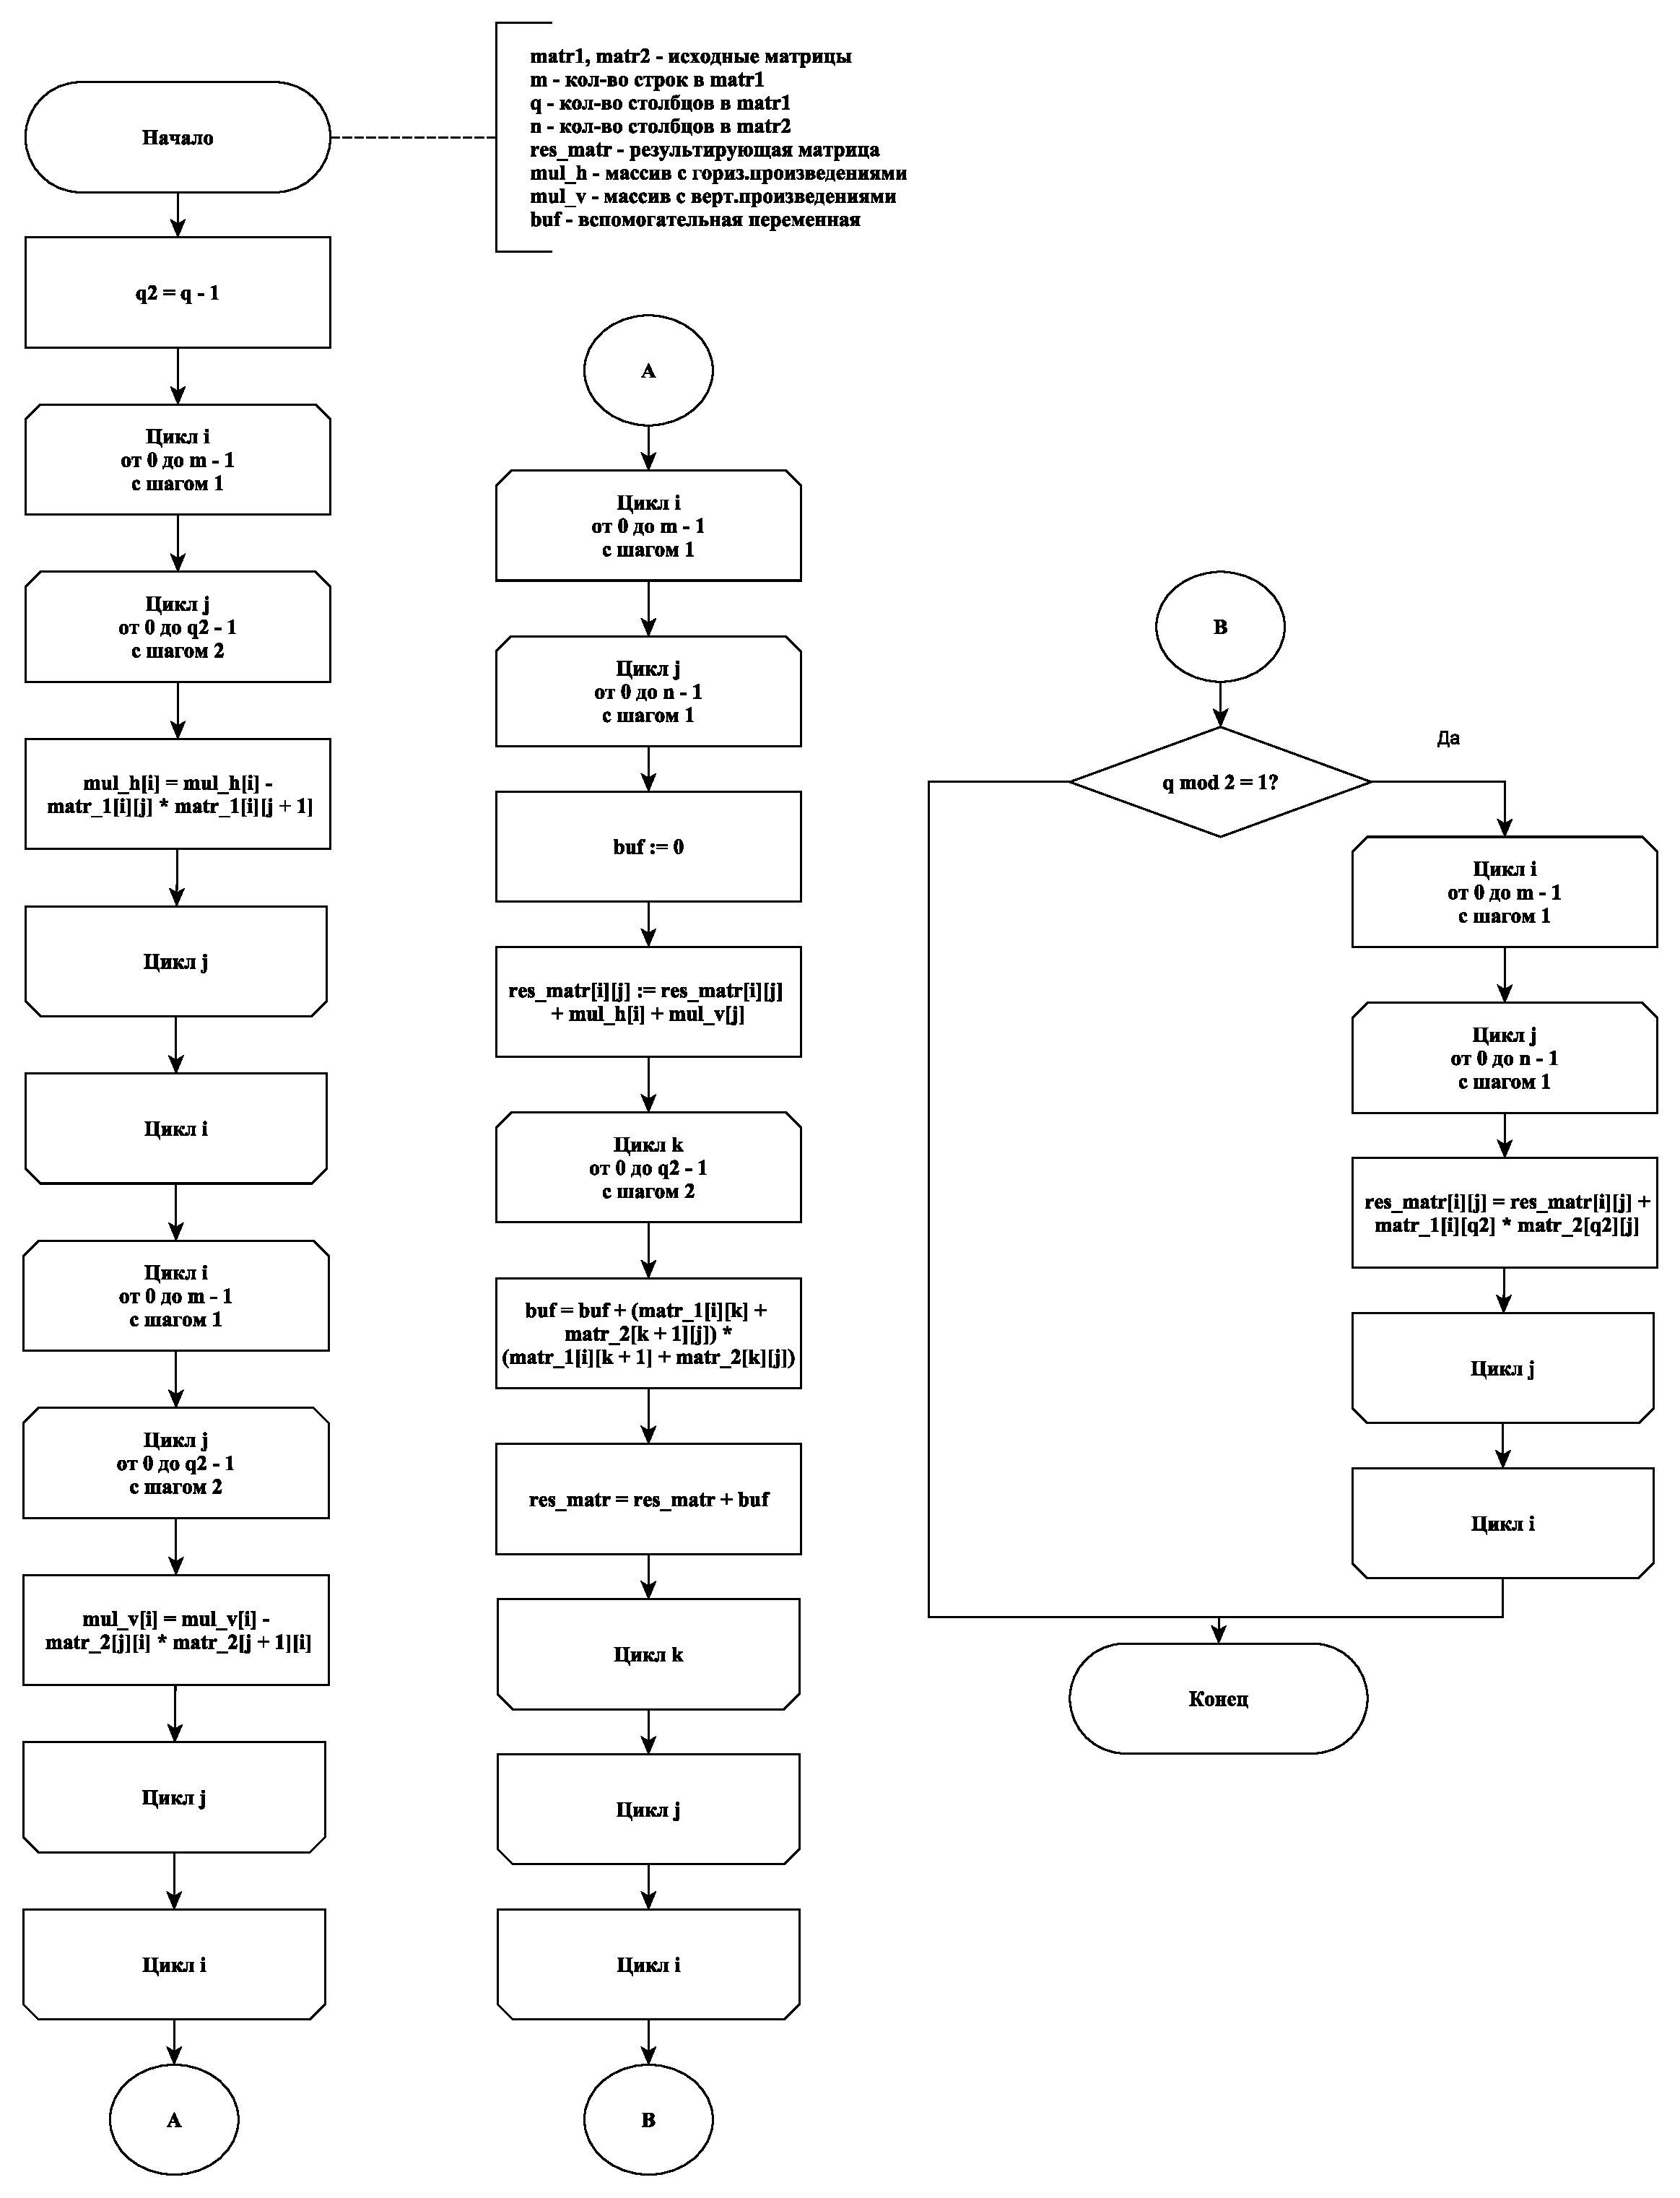
\includegraphics[scale = 0.42]{schema03.pdf}}
	    		\caption{Схема оптимизированного алгоритма умножения матриц по Винограду}
	    		\label{fig:schema_mult_vin_opt}
	    	\end{center}
	    \end{figure}
	    
	 	\newpage
		\mbox{}
		\newpage
		\mbox{}
		\newpage
	    
		\subsection{Сравнительный анализ алгоритмов}
	 \label{fig:an_alg}
		Трудоемкость алгоритмов измеряется в количестве необходимых операций.
		
		Введем модель вычислений:
		\begin{enumerate}
		\item[1)] Базовые операции стоимостью 1: +, -, /, *, =, ==, <=, >= !=, +=, -=, *=, /=, [\:].
		\item[2)] Стоимость цикла:
		\[
		f_{\text{цикла}} = f_{\text{иниц}} + f_{\text{сравн}} + N(f_{\text{тела}} + f_{\text{инкр}} + f_{\text{сравн}}) = 2 + N(f_{\text{тела}} + 2)
		\]
		\item[3)]  Стоимость условного перехода примем за 0, стоимость вычисления условия остается
		
		\end{enumerate}
		Найдем вычислительную сложность алгоритмов для матриц $A[M \times Q]$ и $B[Q \times ~N]$.
		\subsubsection{Стандартный алгоритм}
		По формуле:
		\[
			f = 2 + M(2 + 2 + Q(2 + 2 + N(2 + \underbrace{8}_{[\:]} + \underbrace{1}_{=} + \underbrace{1}_{+} + \underbrace{1}_{*}))),		
		\]
		получаем:
		\[
		f = 13MNQ + 4MQ + 4M + 2.
		\]
		
		\subsubsection{Неоптимизированный алгоритм Винограда}
		Заполнение массива под горизонтальные произведения:
		\[
			f = 2 + M(2 + 3 + \frac{Q}{2}(3 + \underbrace{6}_{[\:]} + \underbrace{1}_{=} + \underbrace{2}_{+} + \underbrace{3}_{*})) = \frac{15}{2}MQ + 5M + 2.		
		\]
		\\
		Заполнение массива под вертикальные произведения (аналогично):
		\[
			f = \frac{15}{2}NQ + 5N + 2.		
		\]
		Непосредственно вычисление произведения матриц:
		\[
		f = 2 + M(2 + 2 + N(2 + \underbrace{8}_{[\:]} + \underbrace{1}_{=} + \underbrace{1}_{-}  + 3 + \frac{Q}{2}(3 + \underbrace{12}_{[]} + \underbrace{1}_{=} + \underbrace{5}_{+} + \underbrace{5}_{*}))) = 
		\]
		\[
		 = 13MNQ + 15MN + 4M + 2.
		\]
		Условный переход:
		\[
		f = 2 + \left [
		\begin{aligned}
		&0,  \text{если}\: Q - \text{четное} \\
		&2 + M(2 + 2 + N(2 + \underbrace{8}_{[\:]} + \underbrace{1}_{=} + \underbrace{3}_{+} + \underbrace{1}_{*})), \text{иначе}
		\end{aligned}
		\right. = \]
		\[ = 2 + \left [
		\begin{aligned}
		&0,  \text{если}\: Q - \text{четное} \\
		&15MN + 4M + 2, \text{иначе}.
		\end{aligned}
		\right. 
		\]
		Итого:
		\[
			f = 13MNQ + \frac{15}{2}MQ + \frac{15}{2}NQ + 15MN + 9M + 5N + 8 + \left [ \begin{aligned}
		&0, \text{если}\: Q - \text{четное} \\
		&15MN + 4M + 2, \text{иначе}.
		\end{aligned}
		\right.
		\]
		
		
		\subsubsection{Оптимизированный алгоритм Винограда}
		Заполнение массива под горизонтальные произведения:
		\[
			f = 2 + M(2 + 2 + \frac{Q}{2}(2 + \underbrace{5}_{[\:]} + \underbrace{1}_{-=} + \underbrace{1}_{+} + \underbrace{1}_{*})) = 5MQ + 4M + 2.	
		\]
		\\
		Заполнение массива под вертикальные произведения ( аналогично горизонтальным):
		\[
			f = 5NQ + 4N + 2.		
		\]	
				Непосредственно вычисление произведения матриц:
		\[
		f = 1 + 2 + M(2 + 2 + N(2 + \underbrace{4}_{[\:]} + \underbrace{1}_{=} + \underbrace{1}_{+} + \underbrace{1}_{buf} + \underbrace{3}_{matr[i][j] = buf} + 
		\]
		\[
		= 2 + \frac{Q}{2}(2 + \underbrace{8}_{[\:]} + \underbrace{1}_{+=} + \underbrace{4}_{+} + \underbrace{1}_{*}))) = 8MNQ + 14MN + 4M + 3.
		\]
				Условный переход:
		\[
		f = 2 + \left [
		\begin{aligned}
		&0, \text{если}\: Q - \text{четное} \\
		&2 + M(2 + 2 + N(2 + \underbrace{6}_{[\:]} + \underbrace{1}_{+=} + \underbrace{1}_{*})), \text{иначе}
		\end{aligned}
		\right. = \]
		\[ = 2 + \left [
		\begin{aligned}
		&0,  \text{если}\: Q - \text{четное} \\
		&10MN + 4M + 2, \text{иначе}.
		\end{aligned}
		\right. 
		\]
		Итого:
				\[
			f = 8MNQ + 5MQ + 5NQ + 14MN + 8M + 4N + 9 + \left [ \begin{aligned}
		&0, \text{если}\: Q - \text{четное} \\
		&10MN + 4M + 2, \text{иначе}.
		\end{aligned}
		\right.
		\]	
	
	\subsubsection{Анализ результатов}
		Оценивать алгоритмы необходимо по самому быстро растущему слагаемому, т. е. по тому в котором одновременно содержатся  три множителя M, N и Q. 
		
		Таким образом самым эффективным оказывается модифицированный алгоритм Винограда: его стоимость $\approx8MNQ$ операций. Стоимость стандартного алгоритма и неоптимизированного алгоритма Винограда составляет $\approx~13MNQ$ операций. Анализ остальных слагаемых стоимостей этих алгоритмов показывает, что стандартный алгоритм эффективнее ($4MQ$ операций против $\frac{15}{2}NQ + \frac{15}{2}MQ  + 15MN$ операций для матриц четной размерности и $4MQ$ операций против $\frac{15}{2}NQ + \frac{15}{2}MQ  + 30MN$ операций для матриц нечетной размерности).
	
	\subsection*{Вывод}
		\addcontentsline{toc}{subsection}{Вывод}
		В данном разделе были представлены схемы стандартного алгоритма умножения матриц и алгоритм умножения матриц по Винограду в двух модификациях: оптимизированный и неоптимизированный.
		
		Был произведен аналитический анализ трудоемкости алгоритмов, в ходе которого выяснилось, что самым эффективным является оптимизированный алгоритм Винограда (стоимость $\approx8MNQ$ операций), менее эффективен стандартный алгоритм (стоимость $\approx13MNQ + 4MQ$ операций). Самым медленным оказался неоптимизированный алгоритм Винограда (стоимость $\approx13MNQ\frac{15}{2}NQ + \frac{15}{2}MQ  + 15MN$ операций).



  
\pagebreak
\newpage         

\section{Технологический раздел}

	В данном разделе будут описаны требования к программному обеспечению и средства реализации, приведены листинг программы и тестовые данные.
	\subsection{Требования к программному обеспечению}
	Входные данные: 
	 \begin{enumerate} 
	 \item[1)] три целых положительных числа - размерности матриц: M, N и Q.
	 \item[2)] две матрицы размера M x Q и Q x N, заполненные целыми числами
	 \end{enumerate}
	
	Выходные данные: матрица размера M x N, полученная в результате умножения исходных, с помощью трех алгоритмов умножения матриц: стандартного, неоптимизированного по Винограду, оптимизированного по Винограду.
	
	На рис. \ref{fig:idef0} приведена функциональная схема вычисления произведения матриц.
        
        \begin{figure}[h!]
        	\begin{center}
        		{\includegraphics[width = \textwidth]{idef0.png}}
        		\caption{Функциональная схема вычисления произведения матриц}
        		\label{fig:idef0}
        	\end{center}
        \end{figure}
        
	
	\subsection{Средства реализации}
	Программа написана на языке С++, т. к. этот язык предоставляет программисту широкие возможности реализации самых разнообразных алгоритмов, обладает высокой эффективностью и значительным набором стандартных классов и процедур. В качестве среды разработки использовался  фреймворк QT 5.13.1.
	
	Для обработки матриц был использован стандартный контейнерный класс std::vector.
	
	Для замера времени выполнения программы использовалась библиотека ctime.
	

    
    \subsection{Листинг программы}
	В листингах \ref{code_std},  \ref{code_vin} и \ref{code_vin_opt} представлены функции стандартного умножения матриц и умножения матриц по Винограду в оптимизированной и неоптимизированной реализациях
	
	\begin{center}
	\begin{lstlisting}[label=code_std, caption={Стандартный алгоритм умножения матриц}]
void mult_matrix_std(Matrix matr_1, Matrix matr_2, Matrix &res_matr) {
    size_t m = matr_1.size();
    size_t q = matr_1[0].size();
    size_t n = matr_2[0].size();

    for(size_t i = 0; i < m; i++) {
        for(size_t j = 0; j < n; j++) {
            for(size_t k = 0; k < q; k++) {
                res_matr[i][j] += matr_1[i][k] * matr_2[k][j];
            }
        }
    }
}
    \end{lstlisting}
    \end{center}  

     
	\begin{lstlisting}[label=code_vin, caption={Неоптимизированный алгоритм Винограда}]
void mult_matrix_vinograd(Matrix matr_1, Matrix matr_2, Matrix &res_matr) {
    size_t m = matr_1.size();
    size_t q = matr_1[0].size();
    size_t n = matr_2[0].size();

    Vector mul_h(m, 0);
    Vector mul_v(n, 0);

    for(size_t i = 0; i < m; i++) {
        for (size_t j = 0; j < q/2; j++) {
            mul_h[i] = mul_h[i] + matr_1[i][j*2] * matr_1[i][j*2 + 1];
        }
    }


    for(size_t i = 0; i < n; i++) {
        for (size_t j = 0; j < q/2; j++) {
            mul_v[i] = mul_v[i] + matr_2[j*2][i] * matr_2[j*2 + 1][i];
        }
    }

    for(size_t i = 0; i < m; i++) {
        for (size_t j = 0; j < n; j++) {
            res_matr[i][j] = - mul_h[i] - mul_v[j];
            for(size_t k = 0; k < q/2; k++) {
                res_matr[i][j] = res_matr[i][j] + (matr_1[i][2*k] + matr_2[2*k + 1][j]) *
                                    (matr_1[i][2*k + 1] + matr_2[2*k][j]);
            }

        }
    }

    if (q % 2 == 1) {
        for(size_t i = 0; i < m; i++) {
            for (size_t j = 0; j < n; j++) {
                res_matr[i][j] = res_matr[i][j] + matr_1[i][q - 1] * matr_2[q - 1][j];
            }
        }
    }
}

\end{lstlisting}


	\begin{lstlisting}[label=code_vin_opt, caption={Оптимизированный алгоритм Винограда}]
void mult_matrix_vinograd_optimiz(Matrix matr_1, Matrix matr_2, Matrix &res_matr) {
    size_t m = matr_1.size();
    size_t q = matr_1[0].size();
    size_t q2 = q - 1;
    size_t n = matr_2[0].size();

    Vector mul_h(m, 0);
    Vector mul_v(n, 0);

    for(size_t i = 0; i < m; i++) {
        for (size_t j = 0; j < q2; j+=2) {
            mul_h[i] -= matr_1[i][j] * matr_1[i][j + 1];
        }
    }


    for(size_t i = 0; i < n; i++) {
        for (size_t j = 0; j < q2; j+=2) {
            mul_v[i] -= matr_2[j][i] * matr_2[j + 1][i];
        }
    }

    for(size_t i = 0; i < m; i++) {
        for (size_t j = 0; j < n; j++) {
            res_matr[i][j] = mul_h[i] + mul_v[j];
            int buf = 0;
            for(size_t k = 0; k < q2; k+=2) {
                buf += (matr_1[i][k] + matr_2[k + 1][j]) *
                                    (matr_1[i][k + 1] + matr_2[k][j]);
            }
            res_matr[i][j] += buf;
        }
    }


    if (q % 2 == 1) {
        for(size_t i = 0; i < m; i++) {
            for (size_t j = 0; j < n; j++) {
                res_matr[i][j] += matr_1[i][q2] * matr_2[q2][j];
            }
        }
    }
}

    \end{lstlisting}  
    
%    
    \subsection{Тестовые данные}
    \label{fig:test_data}

    Программа должна корректно умножать матрицы при следующих входных данных:
\\
\begin{enumerate}
	\item[1)] матрицы $1 \times 1$:
	\[ \begin{bmatrix}
2
\end{bmatrix} \times 
\begin{bmatrix}
3
\end{bmatrix} =
\begin{bmatrix}
6
\end{bmatrix}; \]

	\item[2)] умножение на нулевую матрицу:
	\[ \begin{bmatrix}
1 & 2 \\
3 & 4
\end{bmatrix} \times 
\begin{bmatrix}
0 & 0 \\
0 & 0
\end{bmatrix} =
\begin{bmatrix}
0 & 0 \\
0 & 0
\end{bmatrix}; \]

	\item[3)] умножение на единичную матрицу:
\[ \begin{bmatrix}
1 & 2 \\
3 & 4
\end{bmatrix} \times 
\begin{bmatrix}
1 & 0 \\
0 & 1
\end{bmatrix} =
\begin{bmatrix}
1 & 2 \\
3 & 4
\end{bmatrix}; \]

		\item[4)] умножение(матрицы $2 \times 2$) на матрицу с положительными числами:
\[ \begin{bmatrix}
1 & 2 \\
3 & 4
\end{bmatrix} \times 
\begin{bmatrix}
1 & 2 \\
3 & 4
\end{bmatrix} =
\begin{bmatrix}
7 & 10 \\
15 & 22
\end{bmatrix}; \]

		\item[5)] умножение (матрицы $2 \times 2$) на матрицу с отрицательными числами:
\[ \begin{bmatrix}
1 & 2 \\
3 & 4
\end{bmatrix} \times 
\begin{bmatrix}
-1 & -2 \\
-3 & -4
\end{bmatrix} =
\begin{bmatrix}
-7 & -10 \\
-15 & -22
\end{bmatrix}; \]


		\item[6)] умножение (матрицы $3 \times 3$) на матрицу с положительными числами:
\[ \begin{bmatrix}
1 & 2 & 3 \\
4 & 5 & 6 \\
7 & 8 & 9 
\end{bmatrix} \times 
\begin{bmatrix}
1 & 2 & 3 \\
4 & 5 & 6 \\
7 & 8 & 9 
\end{bmatrix} =
\begin{bmatrix}
30 & 36 & 42 \\
66 & 81 & 96 \\
102 & 126 & 150 
\end{bmatrix}; \]

		\item[7)] умножение (матрицы $2 \times 2$) на матрицу с отрицательными числами:
\[ \begin{bmatrix}
1 & 2 & 3 \\
4 & 5 & 6 \\
7 & 8 & 9 
\end{bmatrix} \times 
\begin{bmatrix}
-1 & -2 & -3 \\
-4 & -5 & -6 \\
-7 & -8 & -9 
\end{bmatrix} =
\begin{bmatrix}
-30 & -36 & -42 \\
-66 & -81 & -96 \\
-102 & -126 & -150 
\end{bmatrix}; \]

	\item[8)] умножение на прямоугольную матрицу с нечётным количеством столбцов:
\[ \begin{bmatrix}
1 & 2 & 3\\
4 & 5 & 6
\end{bmatrix} \times 
\begin{bmatrix}
1 & 2 \\
3 & 4 \\
5 & 6
\end{bmatrix} =
\begin{bmatrix}
22 & 28 \\
49 & 64
\end{bmatrix}; \]

	\item[9)] умножение на  прямоугольную матрицу с чётным количеством столбцов:
\[ \begin{bmatrix}
1 & 2 & 3 & 4\\
5 & 6 & 7 & 8
\end{bmatrix} \times 
\begin{bmatrix}
1 & 2 \\
3 & 4 \\
5 & 6 \\
7 & 8
\end{bmatrix} =
\begin{bmatrix}
50 & 60 \\
114 & 140
\end{bmatrix}; \]

	\item[10)] умножение матриц c большими числами:	
\[ \begin{bmatrix}
1000 & 2000 & 3000 \\
4000 & 5000 & 6000  \\
7000 & 8000 & 9000
\end{bmatrix} \times 
 \begin{bmatrix}
1000 & 2000 & 3000 \\
4000 & 5000 & 6000  \\
7000 & 8000 & 9000
\end{bmatrix} =
\begin{bmatrix}
30000000 & 36000000 & 42000000 \\
66000000 & 81000000 & 96000000 \\
102000000 & 126000000 & 150000000
\end{bmatrix}; \]

	\end{enumerate}
    
    Результаты работы всех трех алгоритмов должны совпадать.
	

		

		
	 
	
	

	
	
	\subsection*{Вывод}
		\addcontentsline{toc}{subsection}{Вывод}
	
	В данном разделе были рассмотрены требования к программному обеспечению, в качестве средств реализации выбраны язык С++ и фреймворк QT версии 5.13.1, приведён листинг программы и тестовые данные. 
	
\pagebreak

\section{Исследовательский раздел}

    
    \subsection{Примеры работы}
        
        На рис. \ref{fig:image_test_1}, \ref{fig:image_test_2}, \ref{fig:image_test_3} и \ref{fig:image_test_4} приведены примеры работы программы для различных входных данных. 
        
        	\begin{figure}[h!]
                \center{\includegraphics[scale = 0.65]{test_1.png}}
                \caption{Пример работы программы для некорректного ввода}
                \label{fig:image_test_1}
            \end{figure}
            
            
            \begin{figure}[h!]
                \center{\includegraphics[scale = 0.65]{test_2.png}}
                \caption{Пример работы программы для матриц $1 \times 1$}
                \label{fig:image_test_2}
            \end{figure}        
        
            \begin{figure}[h!]
                \center{\includegraphics[scale = 0.65]{test_3.png}}
                \caption{Пример работы программы для матриц четной размерности ($2 \times 2$)}
                \label{fig:image_test_3}
            \end{figure}
            
               \begin{figure}[h!]
                \center{\includegraphics[scale = 0.65]{test_4.png}}
                \caption{Пример работы программы для матриц нечетной размерности ($2 \times 3$ и $3 \times 2$)}
                \label{fig:image_test_4}
            \end{figure}
            
    \pagebreak
	\newpage 
	\pagebreak
	\newpage 
            
    \subsection{Результаты тестирования}
    Все тесты из раздела \ref{fig:test_data} успешно пройдены.
    \subsection{Постановка эксперимента}
    
    Необходимо выполнить следующие замеры времени:
    \begin{enumerate} 
        \item Сравнить время умножения матриц стандартным алгоритмом и алгоритмом Винограда в оптимизированной и неоптимизированной модификациях на матрицах размером от $100 \times 100$ до $1000 \times 1000$ с шагом 100.
        \item Провести аналогичное сравнение на матрицах размером от $101 \times 101$ до $1001 \times 1001$ с шагом 100.
    \end{enumerate} 
    
    
    \subsection{Сравнительный анализ на материале экспериментальных данных}
        На рис. \ref{fig:gtaf_1} приводятся графики сравнения времени вычисления алгоритмов при матрицах четной размерности.
        
        \begin{figure}[h!]
            \center{\includegraphics[width = \textwidth]{graf_1.png}}
            \caption{Сравнение времени выполнения алгоритмов на матрицах четной размерности}
            \label{fig:gtaf_1}
        \end{figure}
        
        Как видно, алгоритм оптимизированный алгоритм Винограда выигрывает по быстродействию (на 30\% быстрее неоптимизированного алгоритма Винограда и на 45\% быстрее стандартного алгоритма на матрицах размером $1000 \times 1000$). Хуже себя показал неоптимизированный алгоритм Винограда (на 15\% быстрее стандартного алгоритма на матрицах размером $1000 \times 1000$). Медленнее всех отработал стандартный алгоритм.
        
         На рис. \ref{fig:graf_2} приводятся графики сравнения времени вычисления алгоритмов при матрицах нечетной размерности.
         
        \begin{figure}[h!]
            \center{\includegraphics[width = \textwidth]{graf_2.png}}
            \caption{Сравнение времени выполнения алгоритмов на матрицах нечетной размерности}
            \label{fig:graf_2}
        \end{figure}
        
        Как видно из этих зависимостей, результаты данного замера идентичны результатам предыдущего,эффективность алгоритмов практически не меняется при нечетных размерностях исходных матриц.
        
        Результаты замеров лишь частично совпали с результатами анализа трудоемкости алгоритмов. Оптимизированный алгоритм Винограда, как и ожидалось, оказался самым быстрым, однако стандартный алгоритм уступил в быстродействии неоптимизированному алгоритм Винограда. Такое несоответствие связано, скорее всего с тем, что в разделе \ref{fig:an_alg} мы приняли за 1 трудоёмкость операций, трудоемкость которых на деле отличается (например у операций сложения и умножения).
        
       \subsection*{Вывод}
		\addcontentsline{toc}{subsection}{Вывод}
       В результате тестирования программой были успешно пройдены все заявленные тесты. Эксперименты замера времени показали, что самым эффективным по времени выполнения является оптимизированный алгоритм Винограда, а самым убыточным стандартный алгоритм. Результаты замеров времени не совсем совпали с результатами анализа трудоемкости алгоритмов - стандартный алгоритм, вопреки ожиданиям оказался медленнее неоптимизированного алгоритма Винограда. 
        
    

\pagebreak
\section*{Заключение}
\addcontentsline{toc}{section}{Заключение}
	В ходе работы было выполнено следующее:
	\begin{enumerate}
	
	\item[1)] 
	изучены стандартный алгоритм умножения матриц и алгоритм умножения матриц по Винограду;
	\item[2)] оптимизирован алгоритм Винограда
	\item[3)] применен метод динамического программирования для	реализации указанных
	алгоритмов;
	\item[4)] получены практические навыки реализации указанных алгоритмов: стандартного алгоритма умножения и умножения по Винограду в двух реализациях: оптимизированной и неоптимизированной;
	\item[5)] проведен сравнительный анализ алгоритмов по затрачиваемым ресурсам (времени);
	\item[6)] экспериментально подтверждено различие во временнóй эффективности алгоритмов при помощи разработанного программного обеспечения на материале замеров	процессорного времени на варьирующихся размерностях матриц;
	\item[7)] описаны и обоснованы полученные результаты в отчете о выполненной
	лабораторной
	работе, выполненного как расчётно-пояснительная записка к работе. 
	\end{enumerate}
	
	Аналитический анализ трудоемкости алгоритмов показал, что самым эффективным является оптимизированный алгоритм Винограда (сложность $\approx8MNQ$ операций), сложности стандартного  алгоритма и неоптимизированного алгоритма Винограда оказались практически одинаковыми (сложность $\approx13MNQ$ операций).
	
	Экспериментальный анализ эффективности алгоритмов по времени показал, что самым эффективным является оптимизированный алгоритм Винограда(на 30\% быстрее неоптимизированного алгоритма Винограда и на 45\% быстрее стандартного алгоритма на матрицах размером $1000 \times 1000$). Хуже себя показал неоптимизированный алгоритм Винограда (на 15\% быстрее стандартного алгоритма на матрицах размером $1000 \times 1000$). Медленнее всех отработал стандартный алгоритм. 
	
	Результаты аналитического и эксперементального анализа совпали лишь частично: оптимизированный алгоритм Винограда оказался самым быстрым, а стандартный алгоритм, вопреки ожиданиям, оказался медленнее неоптимизированного Винограда. Такое несоответствие связано, скорее всего с тем, что в разделе \ref{fig:an_alg} мы приняли за 1 трудоёмкость операций, трудоемкость которых на деле отличается (например у операций сложения и умножения).


\pagebreak
\addcontentsline{toc}{section}{Список литературы}
\begin{thebibliography}{4}
\bibitem{makkonell}
Дж. Макконнелл. Анализ алгоритмов. Активный обучающий подход.-
М.:Техносфера, 2009.
\bibitem{matr}
Матрицы и определители [Электронный ресурс]. – Режим доступа: http://matematika.electrichelp.ru/matricy-i-opredeliteli/, свободный – (07.10.2019)

\end{thebibliography}




\end{document} % Конец текста.
